\documentclass[a4paper, 11pt]{article}

\usepackage{kotex} % Comment this out if you are not using Hangul
\usepackage{fullpage}
\usepackage{hyperref}
\usepackage{amsthm}
\usepackage[numbers,sort&compress]{natbib}
\usepackage{graphicx}
\graphicspath{ {images/} }

\theoremstyle{definition}
\newtheorem{exercise}{Exercise}

\begin{document}
%%% Header starts
\noindent{\large\textbf{IS-521 Activity Proposal}\hfill
                \textbf{Name: Kwak Nohyuun}} \\
         {\phantom{} \hfill \textbf{GitHub ID: nohkwak}} \\
%%% Header ends

\section{Activity Overview}
웹은 높은 범용성과 호환성으로 많은 사람들에게 매우 익숙하지만, 보안적으로 많은 취약점을 가지고 있다. 아래 그림은 OWASP에서 발표한 웹 주요 취약점\cite{owasp}을 나타내는데 이번 activity에서는 웹 취약점 가운데 가장 순위가 높은 Injection 취약점을 이해한 후 이 취약점을 자동으로 진단하는 프로그램을 개발하고자 한다. 

\begin{figure}[h]
  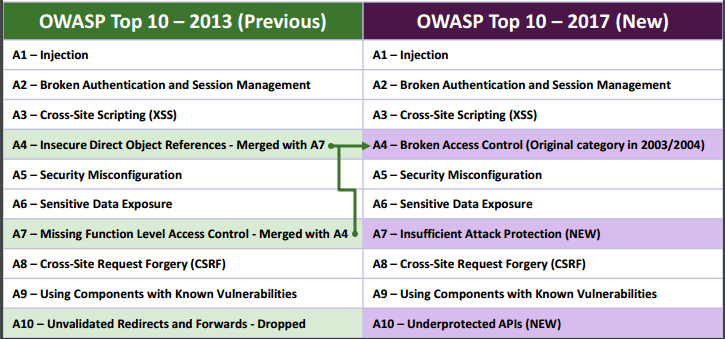
\includegraphics[width=\linewidth]{owasptop.png}
  \caption{OWASP Top 10.}
  \label{fig:owasp}
\end{figure}

\section{Exercises}

\begin{exercise}

WebGoat\cite{webgoat}는 다양한 취약점을 가지고 있는 Web Application Server (WAS) 이다. WebGoat를 설치하고, 설치한 WAS에 접속한다. 

\begin{itemize}
  \item 실행 및 접속 방법 https://github.com/WebGoat/WebGoat/wiki/Running-WebGoat  
\end{itemize}

\end{exercise}

\begin{exercise}

다음 그림과 같이 WAS의 Injection Flaws 메뉴의 하위 메뉴에 있는 문제들을 풀고, 각 문제들에 대해서 다음의 항목들로 간결하게 설명한다. 

\begin{itemize}
  \item 풀이 방법
  \item 풀이 결과 (스크린샷)
\end{itemize}

\begin{figure}[h]
  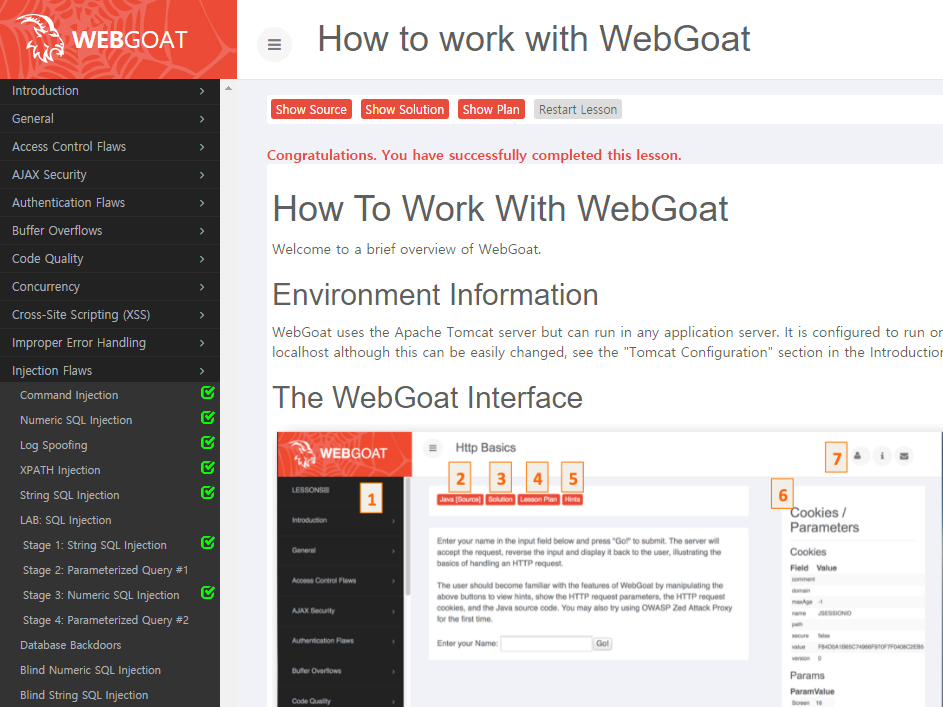
\includegraphics[height=7cm]{webgoat.png}
  \caption{WebGoat.}
  \label{fig:webgoat}
\end{figure}

\end{exercise}

\begin{exercise}

Libcurl\cite{libcurl}은 client-side에서 URL로 http 전송을 할 수 있는 라이브러리이다. 이 라이브러리를 사용하여 위에 설치한 WAS의 Injection Flaws 메뉴의 하위 메뉴 중 Blind Numeric SQL Injection을 자동으로 진단하는 프로그램을 개발한다. 

\begin{itemize}
  \item 실행: ./build/tester http://localhost:8081/WebGoat와 같이 arg로 url을 입력하여 해당 url의 HTML에서 사용자의 입력 및 전송이 가능한 정보를(힌트. form, input 태그) 추출한다. \cite{href} ./build/tester url1  url2  url3 ... 형태의 복수 url도 입력 가능해야 한다.  
  \item 취약점 검사: 위에서 추출한 정보를 바탕으로 입력값을 조작 및 전송하고,\cite{post} 전송 결과들을 바탕으로 취약점의 존재 유무를 판단한다. \cite{getinfo}
  \item 취약점 결과: 취약점 검사 결과, 취약점이 존재하면 아래의 포맷으로 result.txt 파일에 출력한다. \newline  
  Blind Numeric SQL Injection Detected , URL1 \newline 
  Blind Numeric SQL Injection Detected , URL2 \newline
                     ...  
\end{itemize}

Blind Numeric SQL Injection 메뉴와 유사한 구조의 form, input 태그로 구성된 HTML에서도 취약점이 존재하는지 확인할 수 있어야 한다. 

\end{exercise}

\section{Expected Solutions}

위의 Exercise를 수행하고 다음과 같은 결과물을 제출한다. 

\begin{itemize}
  \item ./injection/injection.md : Exercise 2에 해당하는 설명 
  \item ./injection/screenshot/ : 각 문제에 대한 풀이 결과 스크린샷 이미지 

  \item ./tester : Exercise 3에 해당하는 makefile, source, 및 tester.md 파일 
  \item ./tester/Makefile : 실행 파일은 ./build/tester로 생성 되도록 한다. 
  \item ./tester/tester.c :  소스 코드 
  \item ./tester/tester.md  : 스캐너 프로그램에 해당하는 설명 

  \item ./senitizer : (Optional) Exercise 4에 해당하는 proxy 서버 소스 및 senitizer.md 파일 
  \item ./senitizer/senitizer.md : proxy 서버에 해당하는 실행 방법 및 실행 결과에 대한 설명 
\end{itemize}

\bibliography{references}
\bibliographystyle{plainnat}

\end{document}
